\documentclass[a4paper,11pt]{article}
\usepackage[polish]{babel}
\usepackage[latin2]{inputenc}
\usepackage[T1]{fontenc}
\usepackage{anysize}
\usepackage{times}
\usepackage{multirow}
\usepackage{makecell}
\usepackage{graphicx}
\usepackage{tikz}
\usetikzlibrary{calc,through,backgrounds,positioning,fit}
\usetikzlibrary{shapes,arrows,shadows,calendar}
%\marginsize{left}{right}{top}{bottom}
%\marginsize{0cm}{3cm}{3cm}{3cm}

\begin{document}
	\begin{minipage}{5.5cm}
			\begin{tikzpicture}
		\draw (1,0) node[above right] {\textit{Data with cluster assigned}};
		\end{tikzpicture}
	\begin{tabular}{|c|c|c|c|c||c|}
		\hline
		$t$&$a_1$&$a_2$&\dots&$a_k$&$c$\\ \hline \hline
		$t_1$&$v_1^1$&$v_1^2$&\dots&$v_k^1$&$c_1$\\ \hline
		$t_2$&$v_1^2$&$v_2^2$&\dots&$v_k^2$&$c_2$\\ \hline
		\dots&\dots&\dots&\dots&\dots&\dots\\ \hline
		$t_n$&$v_1^n$&$v_2^n$&\dots&$v_k^n$&$c_n$\\ \hline
		\dots&\dots&\dots&\dots&\dots&\dots\\ \hline		
	\end{tabular}
\end{minipage}
\hspace{5mm}
\medskip
\begin{minipage}{2cm}
	\begin{tikzpicture}[scale=1,inner sep=0.4mm]
\draw[-triangle 60] (-1,0) -- (1.5,0);
\draw (0.25,0.5) node[above] {Process};
\draw (0.25,0) node[above] {discovery};
\end{tikzpicture}
\end{minipage}
\hspace{5mm}
\medskip
\begin{minipage}{1.85cm}
	\textit{State graph}
	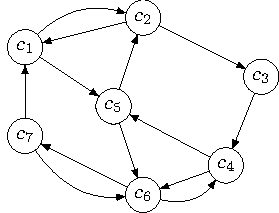
\includegraphics{statesgraph}
\end{minipage}

\end{document}